\section{Thermal Expansion}
\label{sec:thermalExpansion}

\begin{frame}{Thermal Expansion Motivation}
  \begin{itemize}
    \item Strong feedback.
    \item Metallic fuels.
    \item Small active fuel region with high leakage ($\leakage \approx 20\%$).
    \item \gls{ebr-ii} designed and built by \gls{anl} \cite{PlentifulEnergy}.
      \begin{itemize}
        \item Full-power demonstrations from April 1986 \cite{ebriitests}.
        \item \glsentryfull{ulof}.
        \item \glsentryfull{ulohs}.
      \end{itemize}
  \end{itemize}
\end{frame}

\begin{frame}{Material Properties}
  \begin{figure}
    \centering
    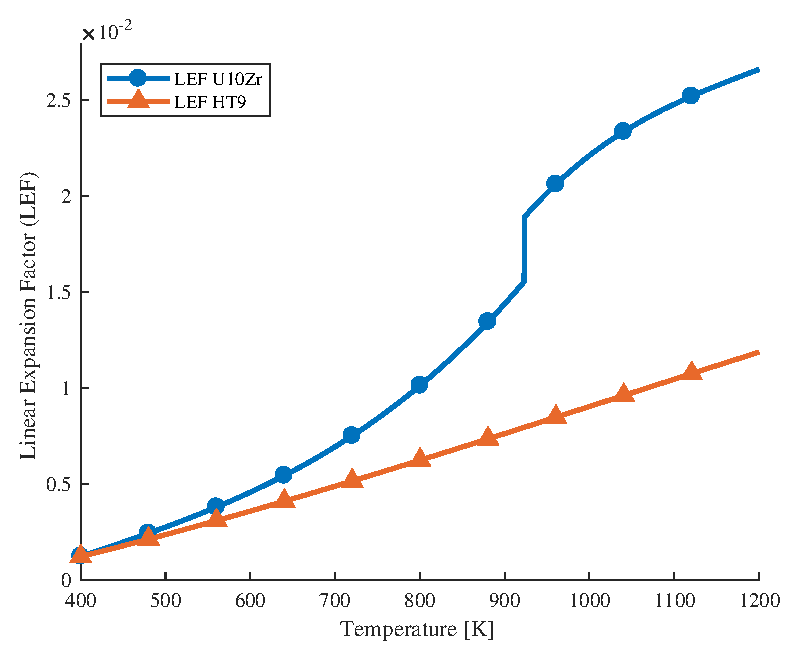
\includegraphics[width=0.7\textwidth]{lef_plot}
    \caption{Linear Expansion Factor for HT9 Steel and U10Zr Fuel.}
    \label{fig:lef_plot}
  \end{figure}
\end{frame}

\begin{frame}{Simplified Thermal Expansion Model}
  \begin{itemize}
    \item User input expansion temperatures $\texpfuel$ and $\texpstruct$.
    \item Leakage effects.
      \begin{itemize}
        \item Finite Elements.
          \begin{itemize}
            \item Radial ($x$ and $y$) directions expanded as structural
              material, HT9 stainless steel.
            \item Axial ($z$) direction expanded as fuel material, U10Zr.
          \end{itemize}
        \item Area fractions.
          \begin{itemize}
            \item Fuel radius expanded as U10Zr.
            \item All other material expanded as HT9 stainless steel.
          \end{itemize}
      \end{itemize}
    \item Density Effects.
      \begin{itemize}
        \item Material densities decreased to conserve quantity of material.
        \item Cross sections decrease proportionally according to $\Sigma = N \,
          \sigma$.
      \end{itemize}
  \end{itemize}
\end{frame}

\begin{frame}{Finite Element Expansion}
  \begin{itemize}
    \item Define radial and axial expansion factors.
      \begin{align}
        \label{eq:lef_r}
        F_r(\texpstruct) &= 1 + \left(\frac{\Delta L}{L}\right)_{\text{HT9}} \\
        \label{eq:lef_a}
        F_a(\texpfuel) &= 1 + \left(\frac{\Delta L}{L}\right)_{\text{U10Zr}}
      \end{align}
    \item Expand all coordinates in the finite element mesh.
      \begin{align}
        \label{eq:expand_x}
        x^H &= x^C \, F_r(\texpstruct) \\
        \label{eq:expand_y}
        y^H &= y^C \, F_r(\texpstruct) \\
        \label{eq:expand_z}
        z^H &= z^C \, F_a(\texpfuel)
      \end{align}
    \item Elements will not overlap or intersect due to uniform expansion
      assumptions.
  \end{itemize}
\end{frame}

\begin{frame}{Arbitrary Volume Expansion}
  \begin{figure}
    \centering
    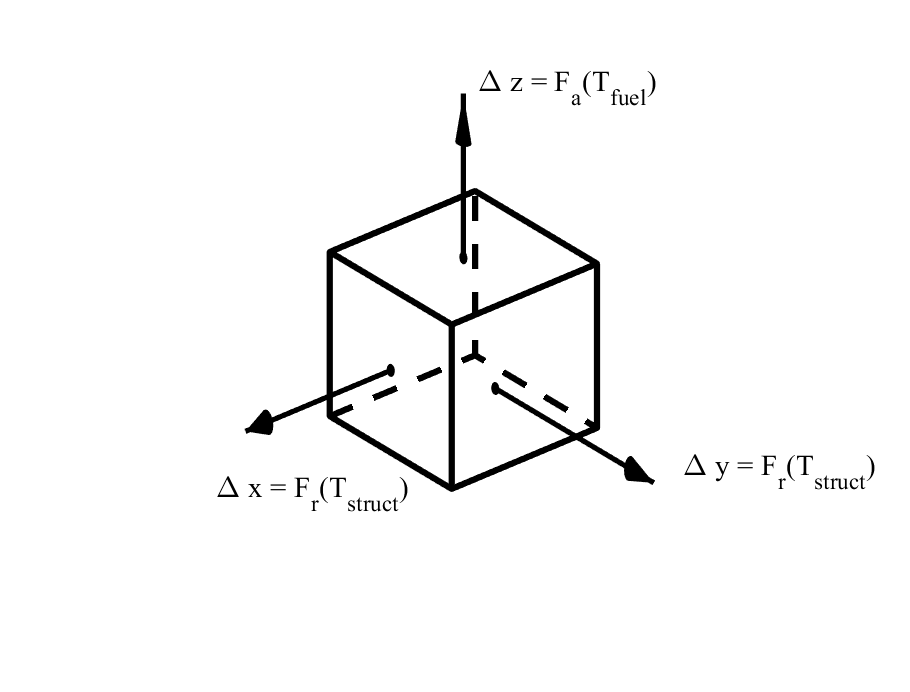
\includegraphics[width=0.9\textwidth]{thexp_figure}
    %\caption{Thermal Expansion of General Volume.}
    \label{fig:thexp_figure}
  \end{figure}
  \vspace{-0.5in}
  \begin{equation}
    \frac{V^C}{V^H} = \frac{1}{(F_r(\texpstruct))^2 (F_a(\texpfuel))}
  \end{equation}
\end{frame}

\begin{frame}{Area Fraction Expansion}
  \begin{itemize}
    \item Dimensions within a hexagonal assembly are expanded.
    \item Area fractions are used for cross section homogenization.
    \item Fuel radius, $R_F$, expanded as U10Zr.
    \item All other dimensions expanded as HT9 stainless steel.
    \item No general formula for expansion of area fractions, calculated
      directly.
  \end{itemize}
  %\begin{figure}
  %  \centering
  %  \subfloat{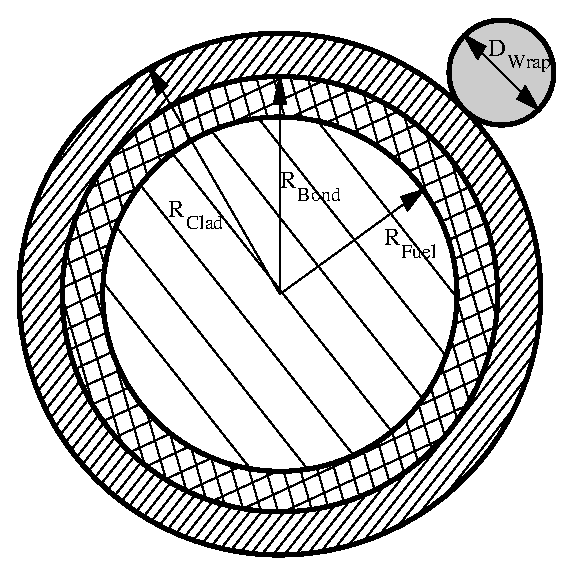
\includegraphics[width=0.35\textwidth]{pin_model}}
  %  \hspace{0.2in}
  %  \subfloat{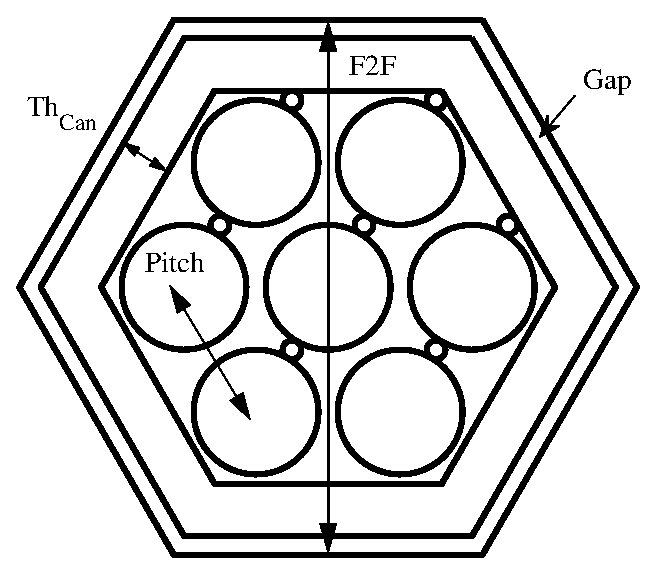
\includegraphics[width=0.35\textwidth]{hex_can}}
  %  \label{fig:assy_geometry}
  %\end{figure}
\end{frame}

\begin{frame}{Conservation of Material \& Cross Section Effects}
  Conservation of number of atoms of species $i$.
  \begin{equation}
    n_i^H = n_i^C
  \end{equation}
  Rewrite the number of atoms using number density and volume.
  \begin{align}
    N_i^H \, V_i^H &= N_i^C \, V_i^C
    %N_i^H &= N_i^C \frac{V_i^C}{V_i^H}
  \end{align}
  Volume $V_i$ can be expressed using element volume and area fraction.
  \begin{equation}
    N_i^H = N_i^C \frac{a_j^C \, V_e^C}{a_j^H \, V_e^H}
  \end{equation}
  Recall the volume ratio.
  \begin{equation}
    N_i^H = N_i^C \frac{a_j^C}{a_j^H} 
      \frac{1}{(F_r(\texpstruct))^2 F_a(\texpfuel)}
  \end{equation}
  Macroscopic cross sections can be updated directly.
\end{frame}

\begin{frame}{Demonstration of Reactor Thermal Expansion}
  \begin{figure}
    \centering
    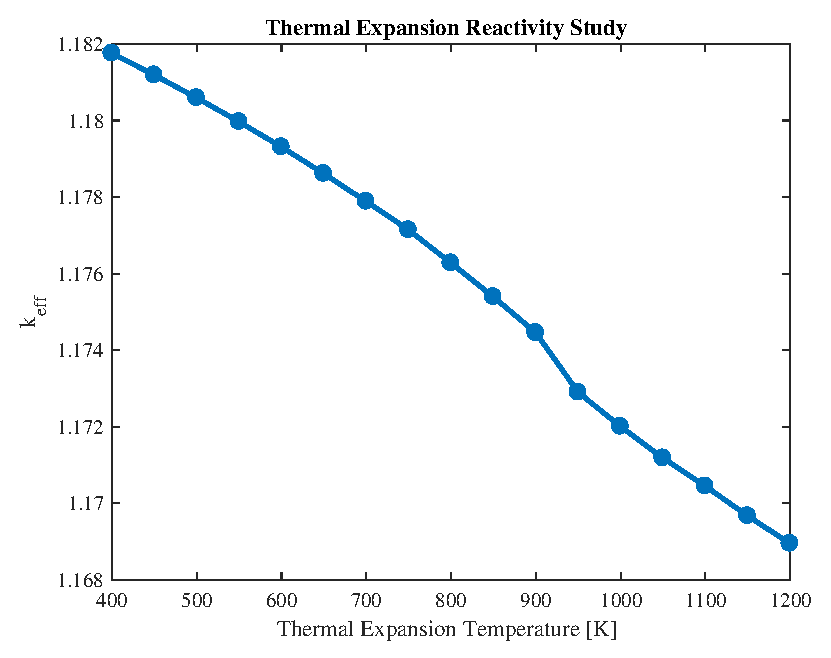
\includegraphics[width=0.7\textwidth]{thexp_study}
    \caption{Effective Neutron Multiplication Factor as a Function of 
      Thermal Expansion Temperature.}
    \label{fig:thexp_study}
  \end{figure}
\end{frame}
